%====================================================================================================
\chapter{The Athena Framework} \label{ch:Athena}
%====================================================================================================
The ATLAS software framework supports experimental data transformation, Monte Carlo generation and simulation, and downstream analysis of the ATLAS detector data. The framework includes several projects, the most comprehensive one among them forms the basis of Athena~\cite{ATLAScomputing2025}, a general-purpose offline software framework based on Gaudi architecture. This chapter briefly introduces the Gaudi architecture, followed by an overview of the Athena framework built on it. Besides, new development to multi-threaded Athena are also presented.
%====================================================================================================
\section{The Gaudi Architecture} \label{sec:Gaudi}
%====================================================================================================
The Large Hadron Collider (LHC) generates petabytes of raw data each year. To extract meaningful physics insights, these data must be processed through multiple stages such as reconstruction of kinematical variables by detector signals, filtering and selection of data of interest, and offline analysis for physics purposes. Since the experiments are planned to continue for many years, it is crucial to anticipate evolving software requirements and advancements in the underlying technologies. Therefore, the software must be designed with enough flexibility and adaptability, allowing it to accommodate these changes and remain maintainable over extended periods of operation.

To address that, a new object-oriented software framework for High Energy Physics, Gaudi, was developed \cite{Gaudi}. Originally designed for the LHCb experiment, Gaudi provides a modular and flexible environment for building various data-processing applications across various computing platforms. As the core of the framework, Gaudi is based on a well-defined architecture that specifies the main components and their interactions. Figure~\ref{fig:Gaudi_object_diagram} shows the major components of the Gaudi software architecture. The architecture of the Gaudi framework is introduced in the following.

\begin{figure}[htbp]
  \centering
  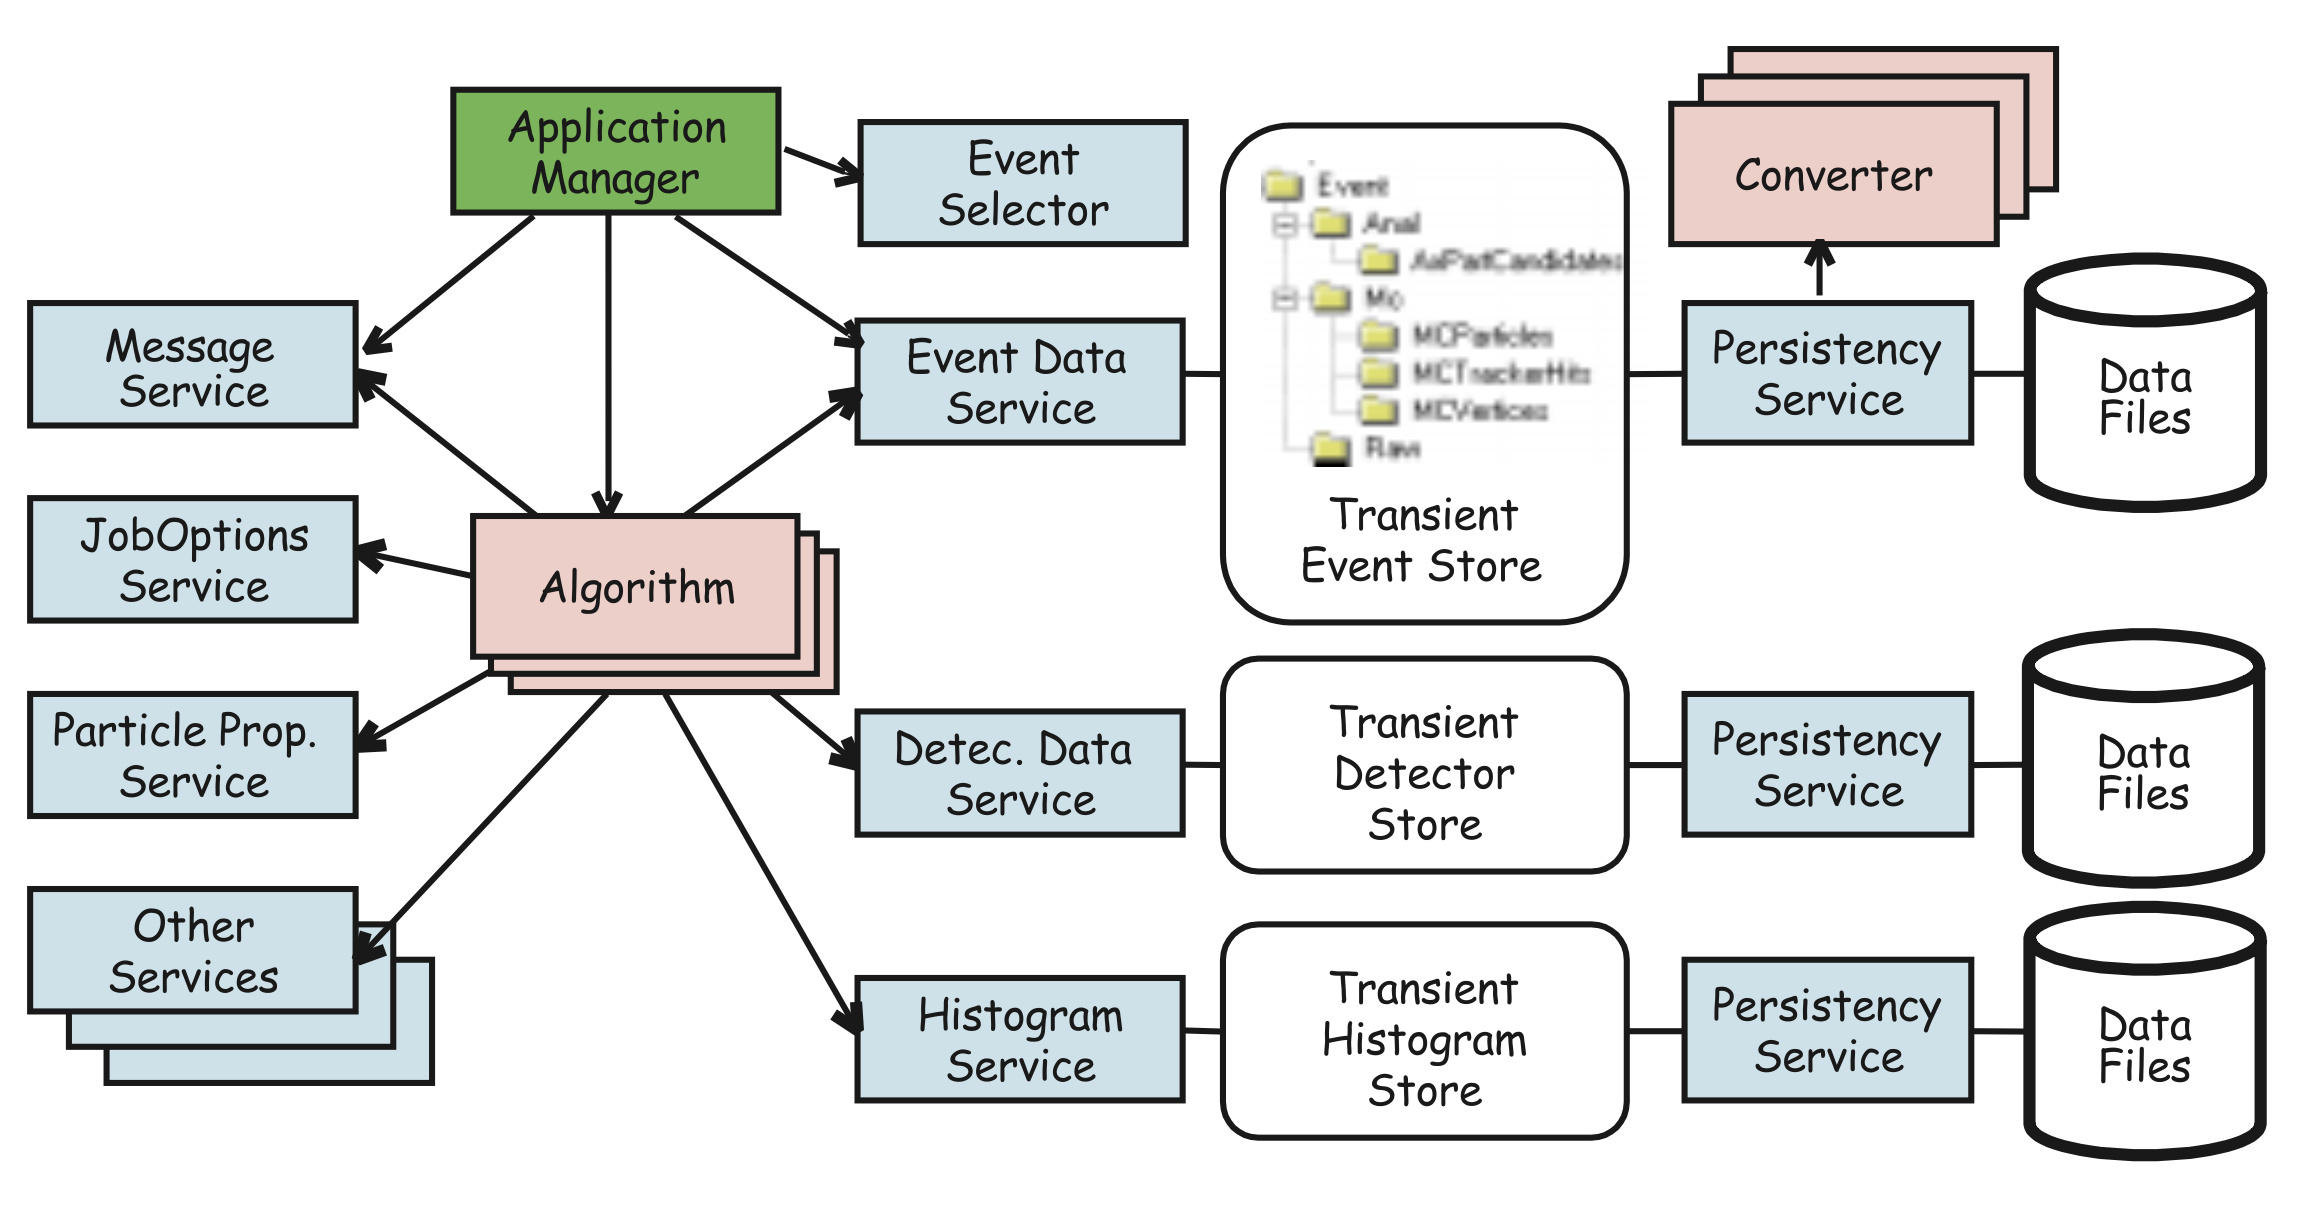
\includegraphics[width=0.9\textwidth]{figs/chapter3/Gaudi_object_diagram.png}
  \caption{Object diagram of the Gaudi architecture \cite{Gaudi}.}
  \label{fig:Gaudi_object_diagram}
\end{figure}

%====================================================================================================
\subsection{Algorithms and Application Manager}
%====================================================================================================
In event data processing, the core functionality is realized through \textit{physics algorithms}, which are encapsulated as modular components referred to as algorithms. The algorithms implement a standard set of interfaces, allowing them to be invoked (called) without requiring knowledge of their internal workings. More complex functionalities can be constructed by composing simpler algorithms. Overseeing the algorithm execution flow is the \textit{application manager}, responsible for instantiating and orchestrating algorithms as needed.

The execution of algorithms follows an explicit scheduling model. A complex algorithm manages the order of their sub-algorithms to ensure correct results. If a particular algorithm relies on data produced by another, it becomes necessary to explicitly define the execution order to maintain consistency. Figure~\ref{fig:Gaudi_dataflow} shows how proper sequencing and the use of a transient data store (see below) enables coherent data flow across different algorithmic stages.

\begin{figure}[htbp]
  \centering
  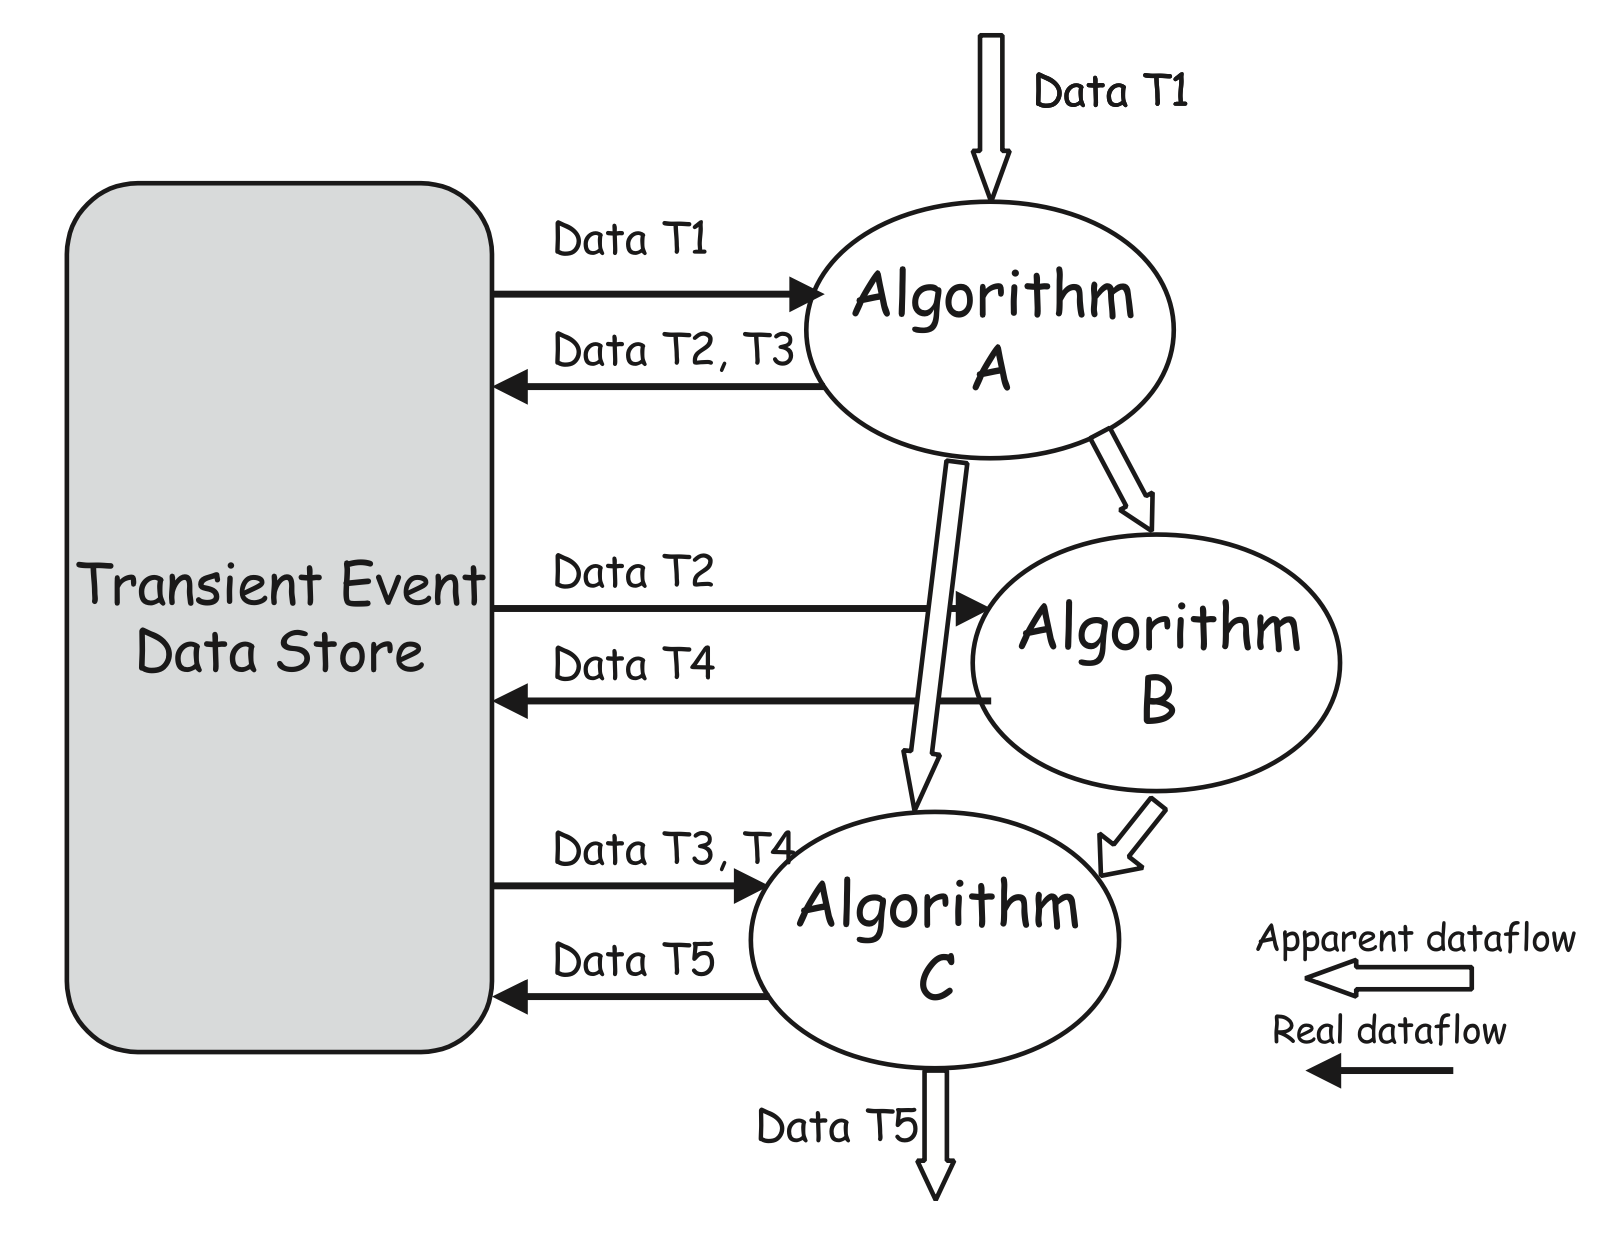
\includegraphics[width=0.8\textwidth]{figs/chapter3/Gaudi_dataflow.png}
  \caption{A demonstration of achieving the intended dataflow via structured scheduling of algorithmic components \cite{Gaudi}.}
  \label{fig:Gaudi_dataflow}
\end{figure}

%====================================================================================================
\subsection{Transient data stores}
%====================================================================================================
The Gaudi framework uses several \textit{transient data stores} to manage the exchange and lifecycle of data between algorithms. They are applied depending on the nature and lifetime of the data:

\begin{itemize}
    \item \textbf{Transient Event Store} handles event data that are valid only during the processing of a single event.
    \item \textbf{Transient Detector Store} contains data that describe various aspects of the behavior of the detector, which typically persist across many events.
    \item \textbf{Transient Histogram Store} holds statistical data, and generally lasts across the processing of a complete job.
\end{itemize}

The purpose of the Transient Store is to minimize the coupling between algorithms and data objects. Algorithms can store intermediate results into the transient store, and other algorithms can access this data later without needing to know how it was produced. In this way, different algorithms communicate indirectly via a shared data space. The Transient Store serves as an intermediate buffer between different data representations, responsible for conversion from transient data to persistent or graphical formats.
%====================================================================================================
\subsection{Services}
%====================================================================================================
Services in the Gaudi framework are a category of components that provide all the services and functionalities required by the algorithms, either directly or indirectly. This architectural approach releases many software routine tasks from the algorithm developer, enabling them to focus on physics data processing logic. These services are briefly introduced as below, some of which could be seen in Figure~\ref{fig:Gaudi_object_diagram}.

Some services are responsible for managing transient data stores, including the event data service and detector data service, etc. These services simplify data access and ensure efficient communication between different components of the framework. In addition, the different persistency services provide the functionalities in managing the transformation of data between transient and persistent representations. These transformations rely on specific \textit{converters}, which are capable of converting a given data object into its appropriate format. Auxiliary services are also provided by Gaudi, such as the job options service, the message service, particle properties service and other services such as visualisation and event selectors.

%====================================================================================================
\section{Athena}
%====================================================================================================
Although Gaudi was originally developed within the context of the LHCb experiment~\cite{LHCb_tech}, it was designed to be highly customizable and adaptable to various tasks, making it suitable for integration into the software environments of other experiments. The Gaudi framework is now shared by many particle physics experiments, in which the ATLAS is included \cite{CHEP2004}. Here, a brief overview of ATLAS control framework based on Gaudi architecture, \textit{Athena}, is presented.

Athena is the object oriented control framework used by the ATLAS experiment at CERN. It is developed in C++, and is designed with a modular component architecture, consisting of a series of packages covering all the main processes along the data flow. It is also supplemented by external libraries such as POOL, a data storing service, and Geant, a software package for MC simulation.
The framework enforces a clear separation between transient and persistent data. Components access data through abstract interfaces rather than direct access to the implementation. This allows individual components to be easily replaced or updated as technologies advance. Athena comprises the ATLAS specific extensions to Gaudi, which includes:

\begin{itemize}
    \item \textbf{StoreGate} - a transient data store used for exchanging information between algorithms during processing~\cite{AthenaStoreGate}.
    \item \textbf{Interval of Validity Service (IOVSvc)} - handles time-dependent conditions and detector data.
    \item \textbf{Pileup} - supports the simulation of multiple interactions within a single bunch crossing to approach realistic experimental conditions.
    \item \textbf{History Service} - maintains a multi-level record of data provenance, enabling traceability and reproducibility of reconstructed data.
    \item \textbf{Python Scripting} - provides configuration and interactive control of Athena components based on Python.
\end{itemize}

In a data processing flow on Athena, dynamically loadable components are employed, leading to the concepts of Algorithms, Services, and Tools introduced in Section~\ref{sec:Gaudi}. The processing flow is illustrated as Figure~\ref{fig:Athena_process}. 

Algorithms operate on data reside in a shared event store, where they retrieve and store objects identified by type and a string key. In principle, each Algorithm is stateless with respect to event data and communicates with others solely through the event store. Services are shared resources accessed by multiple components, such as the event store itself, error logging, and random number generation. Tools act as auxiliary components and can be uniquely owned by Algorithms, Services, or even other Tools. Each of the three component types, namely the Algorithms, Services and Tools, supports the declaration of configurable properties, allowing consistent initialization as part of the job setup phase.

\begin{figure}[htbp]
  \centering
  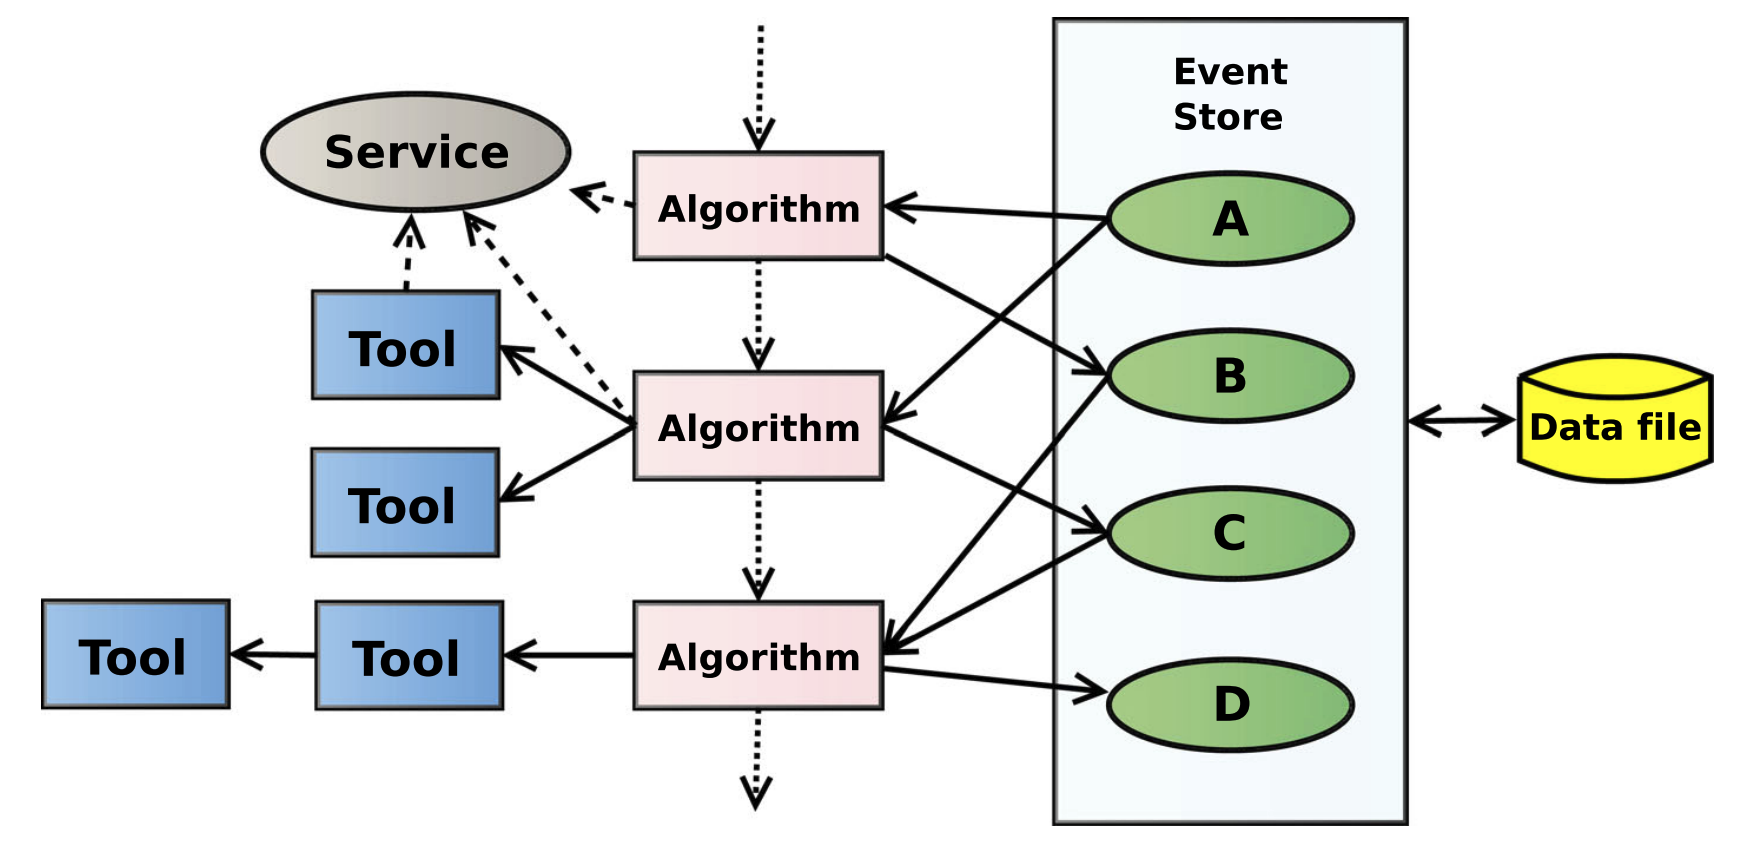
\includegraphics[width=0.85\textwidth]{figs/chapter3/Athena_process.png}
  \caption{Schematic of Athena processing flow. The solid lines on the right indicate data flow, on the left they indicate ownership. The dotted line indicates the application control flow. The dashed lines indicate a non-owning reference between components \cite{ATLAScomputing2025}.}
  \label{fig:Athena_process}
\end{figure}


%====================================================================================================
\section{Multi-threaded Developments for Athena}
%====================================================================================================
The Athena framework was initially developed in the early 2000s, when the processing speed is determined mainly by that of single-core CPU clock speeds. As such, it was fundamentally designed for serial event processing. During LHC Run~2, 2015 to 2018, increasingly demanding computing conditions were addressed through the development of \textit{AthenaMP}~\cite{AthenaMP}, a multi-process version of Athena. AthenaMP operates by forking multiple worker processes from a primary process after the initialization phase. These workers run the event loop in parallel, allowing large static memory structures, such as detector geometry and magnetic field maps, to be shared via the Linux kernel’s copy-on-write mechanism.

However, this approach also presents limitations. Minor changes in memory, such as modifying a single bit, can cause entire memory pages to become unshared, negating the benefits of memory sharing. Furthermore, the C++ memory model does not allow for fine control over which data are assigned to which physical pages. In addition, with the further evolution of the LHC, event complexity and data acquisition rates are expected to increase significantly. These challenges motivated the development of \textit{AthenaMT}, a multi-threaded version of the Athena framework in LHC Run~3 phase. In multi-process (MP) parallelism, worker processes are forked from a primary process a pre-configured stage in execution (e.g., before or after the first event is processed). After forking, workers share memory pages allocated in the primary process but otherwise execute independently in parallel. Each worker has its own private memory region and produces output separately, requiring a dedicated post-processing step for output merging. The event throughput and memory usage comparison between AthenaMP and AthenaMT are shown in Figure~\ref{fig:AthenaMT_throughput} and Figure~\ref{fig:AthenaMT_memory}, respectively.

\vspace{1em}
\begin{figure}
    \centering
    \begin{minipage}{0.49\textwidth}
        \centering
        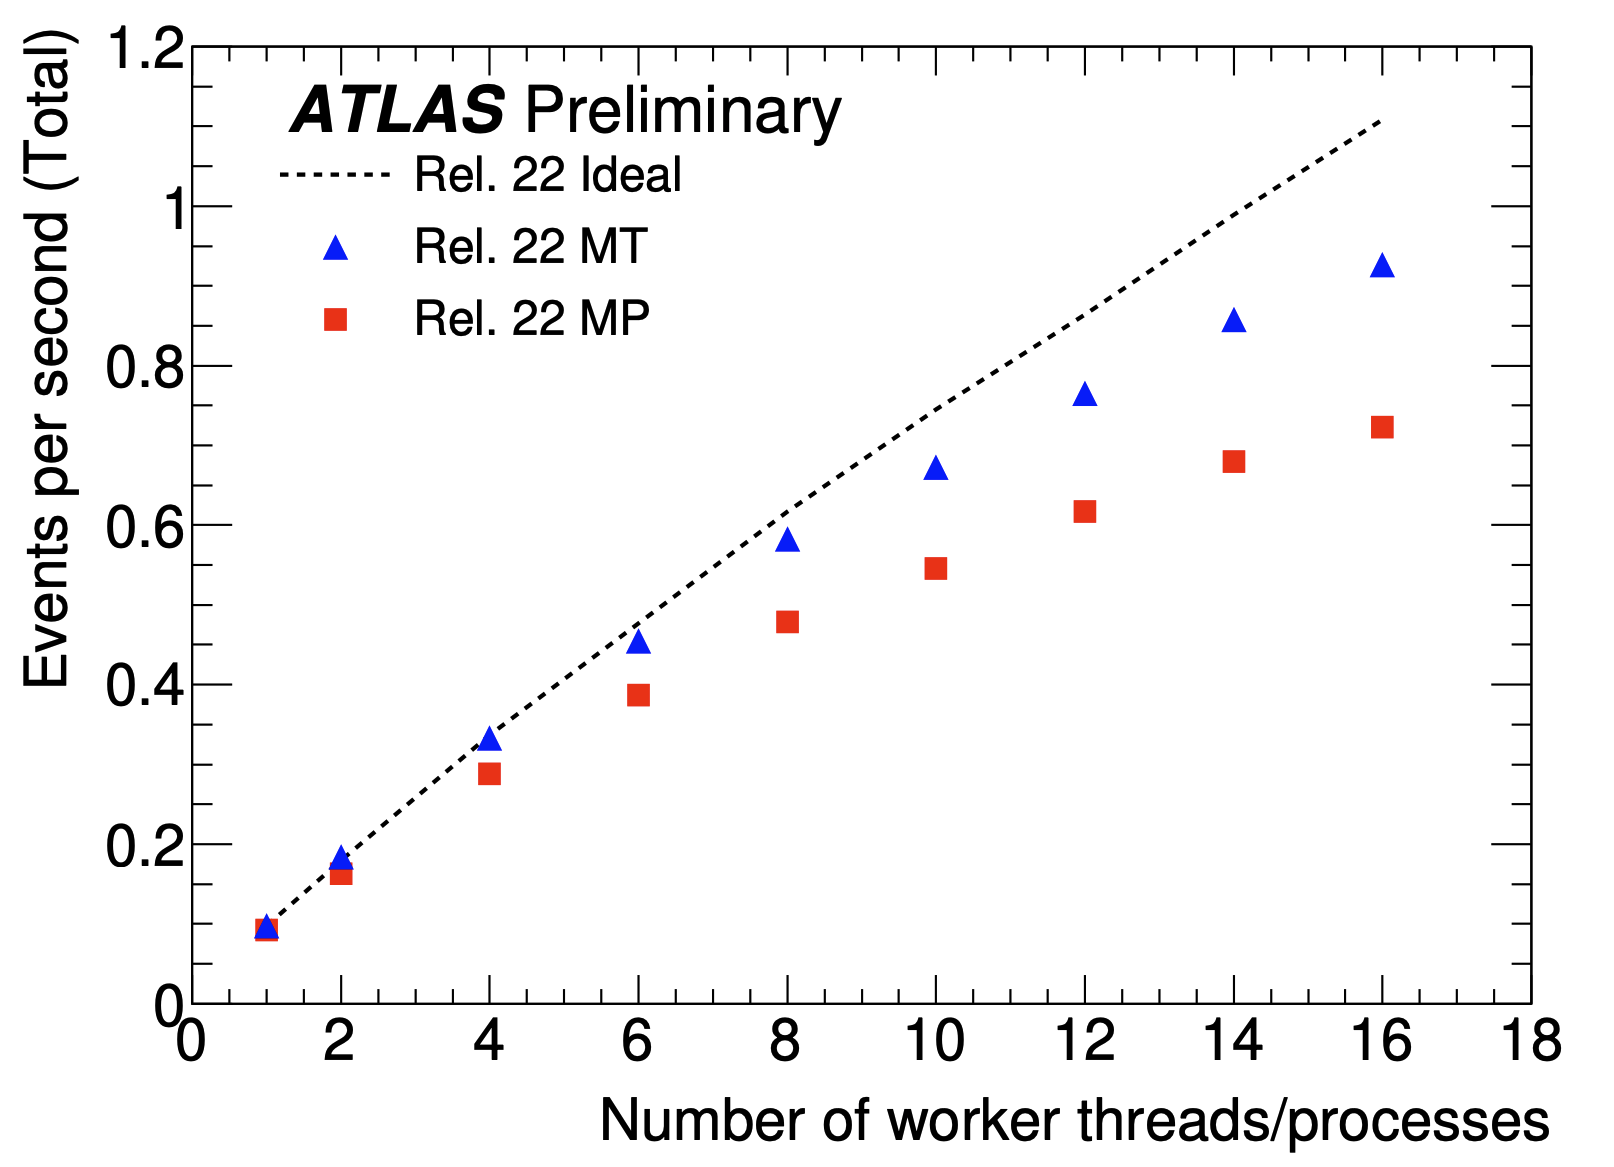
\includegraphics[width=\linewidth]{figs/chapter3/AthenaMT_throughput.png}
        \caption{Comparison of event throughput of the ATLAS reconstruction as a function of number of threads/processes in Athena release 22 \cite{AthenaMT&MP}.}
        \label{fig:AthenaMT_throughput}
    \end{minipage}
    \hfill
    \begin{minipage}{0.49\textwidth}
        \centering
        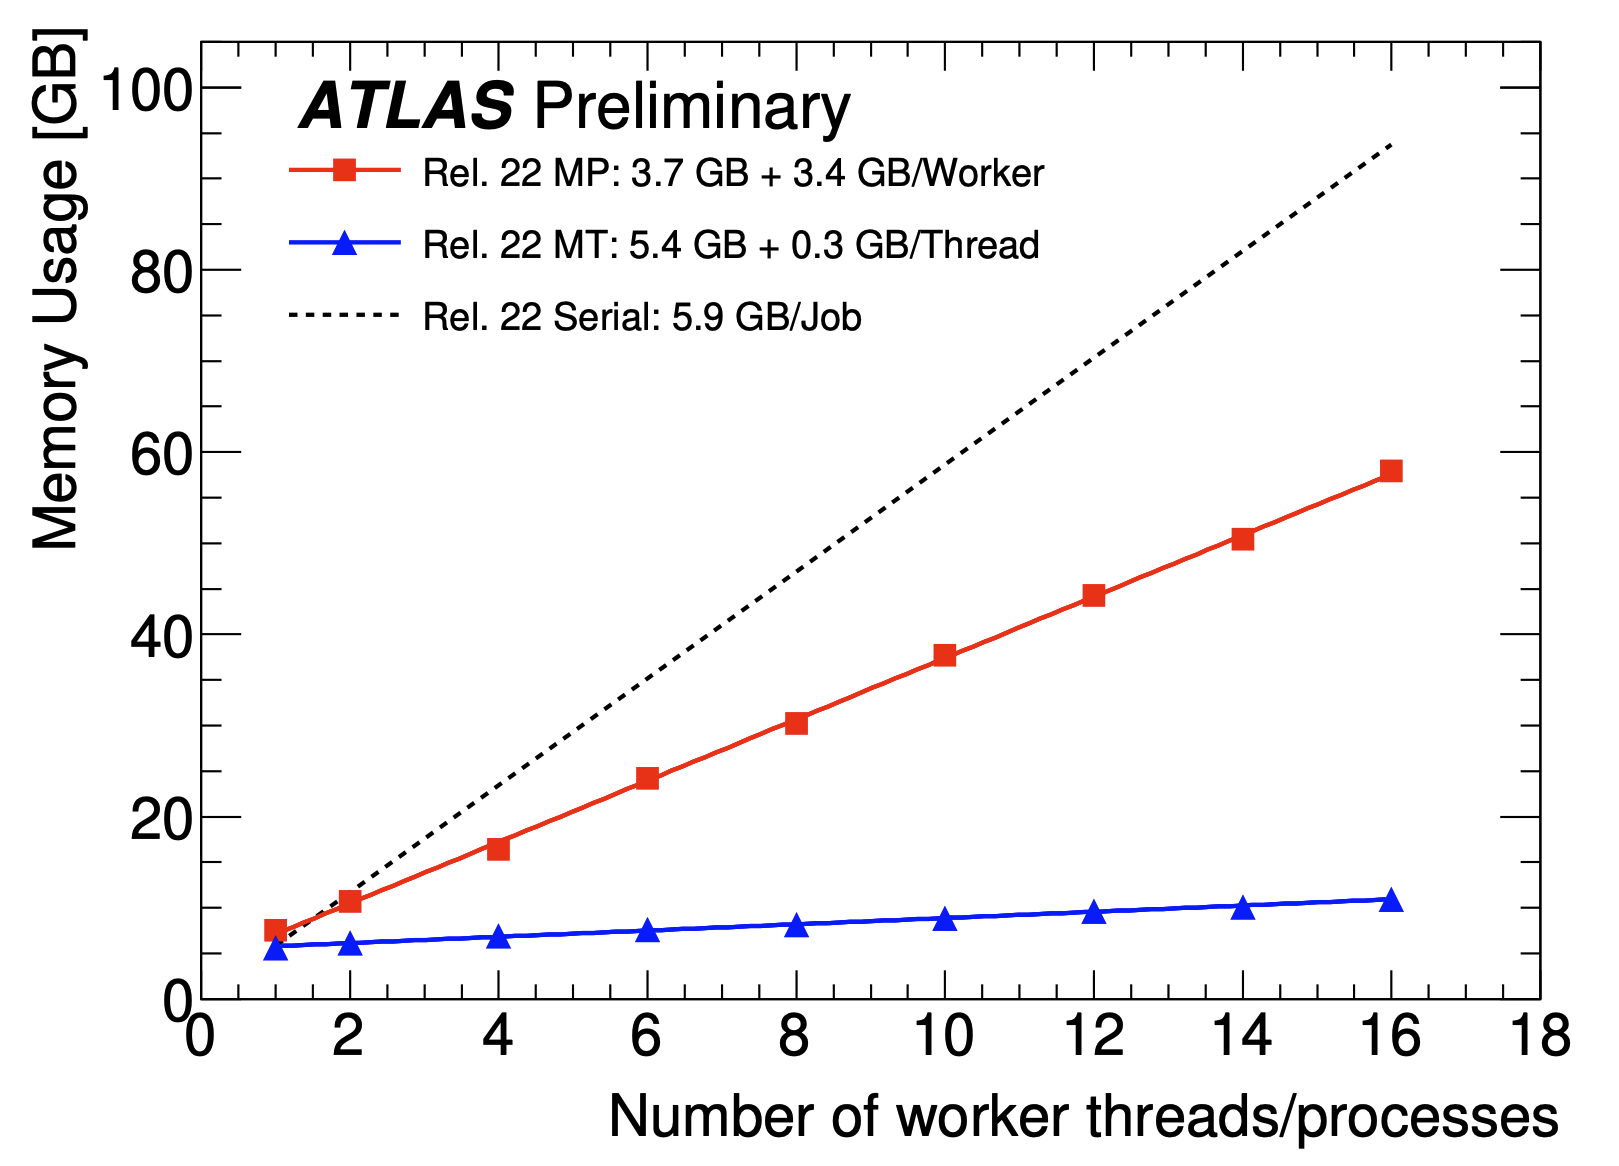
\includegraphics[width=\linewidth]{figs/chapter3/AthenaMT_memory.png}
        \caption{Comparison of memory usage of the ATLAS reconstruction as a function of number of threads/processes in Athena release 22 \cite{AthenaMT&MP}.}
        \label{fig:AthenaMT_memory}
    \end{minipage}
\end{figure}

The multi-threaded framework adopted in Run~3 sets some new requirements for software development and code design \cite{ATLAScomputing2025}. In the Athena implementation of muon trigger simulation for Phase-II upgrade, which will be discussed in Chapter~\ref{ch:L0MuonS1TGC}, several adaptations were made compared to non-threaded code in order to ensure safe and consistent behavior under multi-threaded environment:

\begin{enumerate}
  \item \textbf{Event and conditions data are accessed via handles.} \\
  All data access is performed through \textit{handles}, avoiding direct use of non-thread-safe caching or back-channel communication. For example, \texttt{SG::ReadHandleKey} and \texttt{SG::WriteHandleKey} defined in the \texttt{StoreGate} class, are used for retrieving and writing data in StoreGate by using ``Keys'' corresponding to the specific data being accessed, preventing race conditions when data is accessed concurrently by different threads.
  
  \item \textbf{Unique object for each process are applied.} \\
  Each algorithm instance writes to a separate data object. In a multi-threaded environment, event data must only be modified by the processing thread. Therefore, this implementation uses unique objects for each process, avoiding appending to or modifying existing data objects.
  
  \item \textbf{Non-const data structure are avoided.} \\
  The non-const data structures, including functions and variables, are considered unsafe in multi-threaded processes, since it may cause data conflict if a non-const data structure was shared in several threads. Shared non-const static data can introduce data conflicts and non-determinism across threads.
  
  \item \textbf{Thread-safe Services are used.} \\
  All Services used in this implementation are explicitly thread-safe. Since Services are global components accessed by multiple algorithms, they are either stateless, properly synchronized (e.g., via status locking), or designed to operate with thread-local data.
\end{enumerate}

Through these measures, the implementation can be operated with thread safety on the Athena multi-threaded environment.